\documentclass[a4paper, brazil]{article}
\usepackage[utf8]{inputenc}

\usepackage[cm]{fullpage}
\usepackage{pacotesLaTeX}

\author{Thales Freitas Macêdo \\ DRE: 115 162 177}
\title{LISTA 3}

\begin{document}

\maketitle

\section{Exercício 1}

\begin{figure}[ht]
\centering
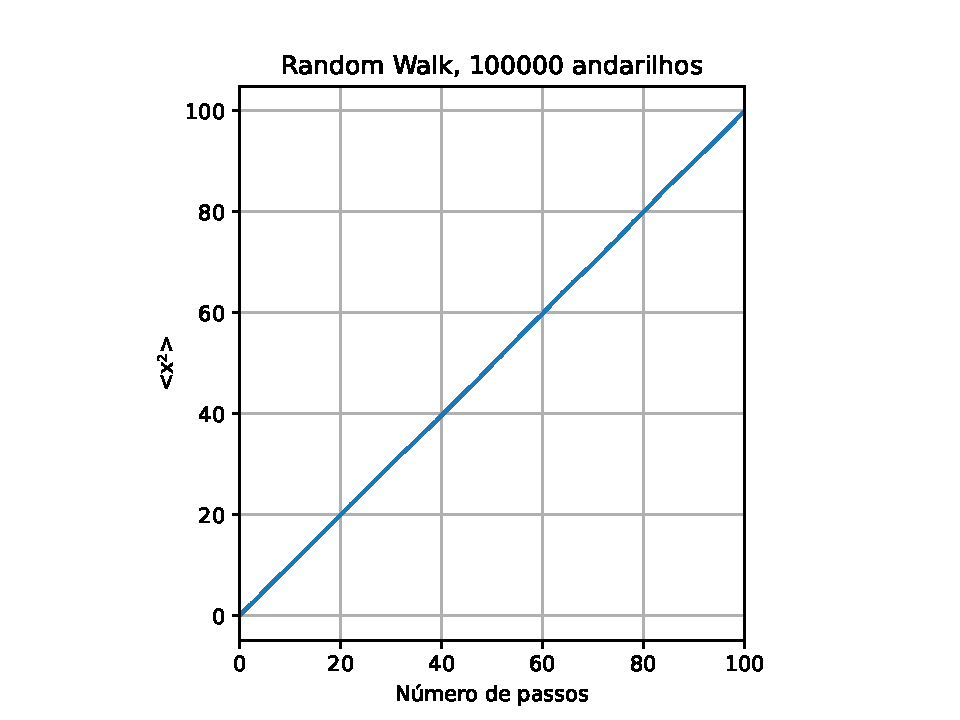
\includegraphics[width=\textwidth]{fig_1.pdf}
\caption{Gráfico de \( \expval{x^2} \) em função do número de passos (tempo) para o Random Walk com 100000 andarilhos.}\label{fig1}
\end{figure}

A figura \ref{fig1} apresenta o gráfico de \( \expval{x^2} \) em função do número de passos (tempo) para o Random Walk com 100000 andarilhos.
Após realizar um ajuste linear for mínimos quadrados, obtive o valor de \num{0.49982} para o coeficiente de difusão \( D \).

\newpage
\section{Exercício 2}

\begin{figure}[ht]
\centering
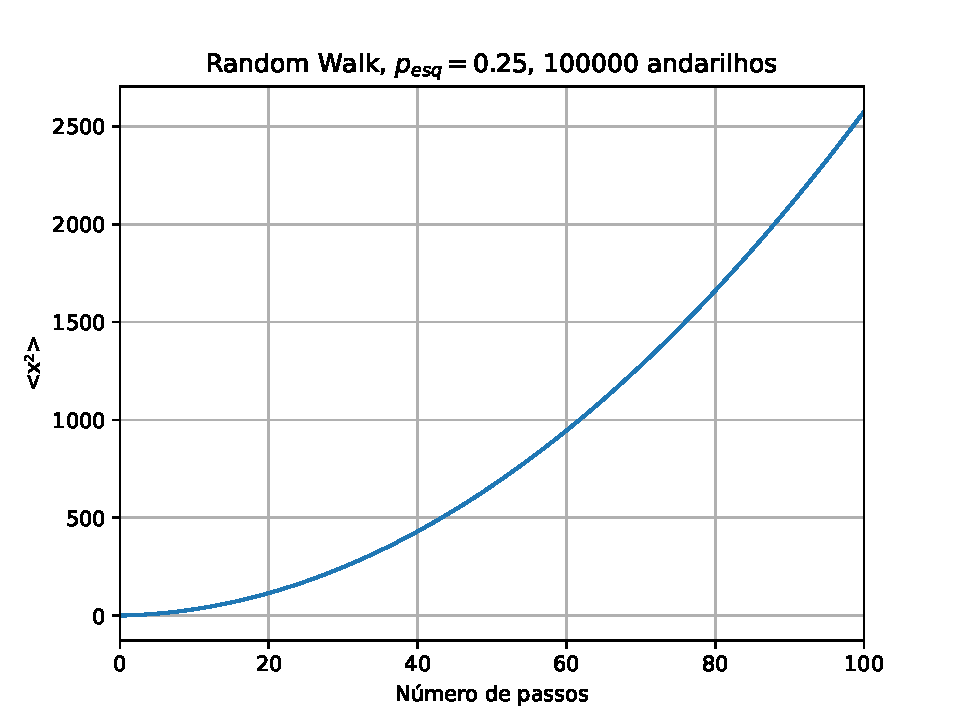
\includegraphics[width=\textwidth]{fig_2.pdf}
\caption{Gráfico de \( \expval{x^2} \) em função do número de passos (tempo) para o Random Walk com 100000 andarilhos, onde a probabilidade do andarilho ir para a esquerda é \num{0.25}.}\label{fig2}
\end{figure}

A figura \ref{fig2} apresenta o gráfico de \( \expval{x^2} \) em função do número de passos (tempo) para o Random Walk com 100000 andarilhos, onde a probabilidade do andarilho ir para a esquerda é \num{0.25}.
O comportamento não é mais difusivo, já que \( \expval{x^2} \) não é mais linear com o tempo.

\newpage
\section{Exercício 3}

\begin{figure}[ht]
\centering
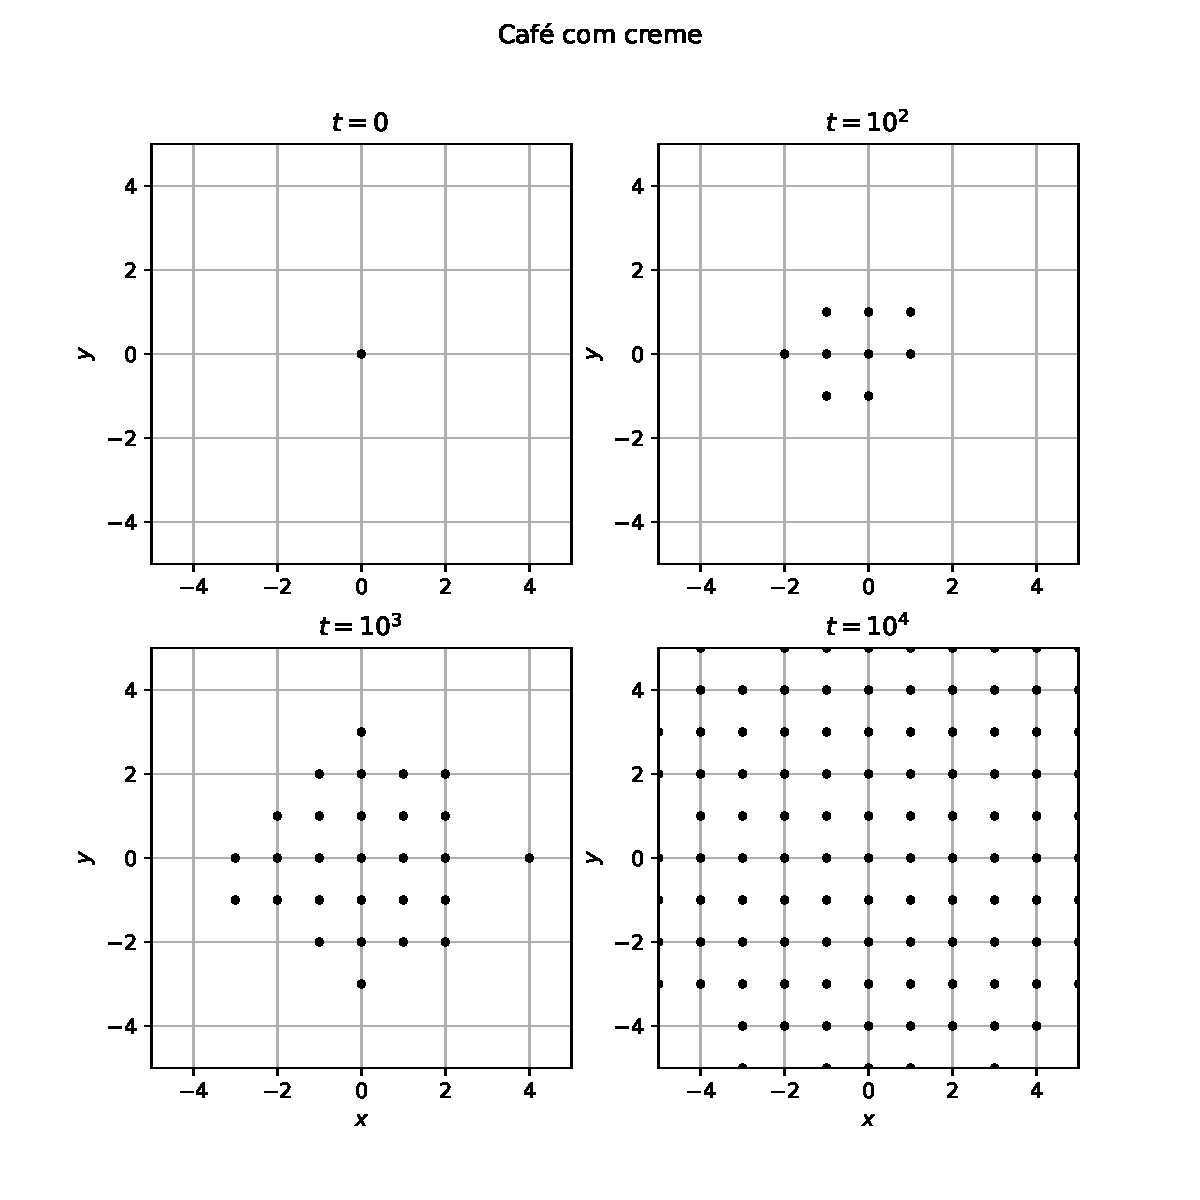
\includegraphics[width=0.4\textwidth]{fig_3a.pdf}
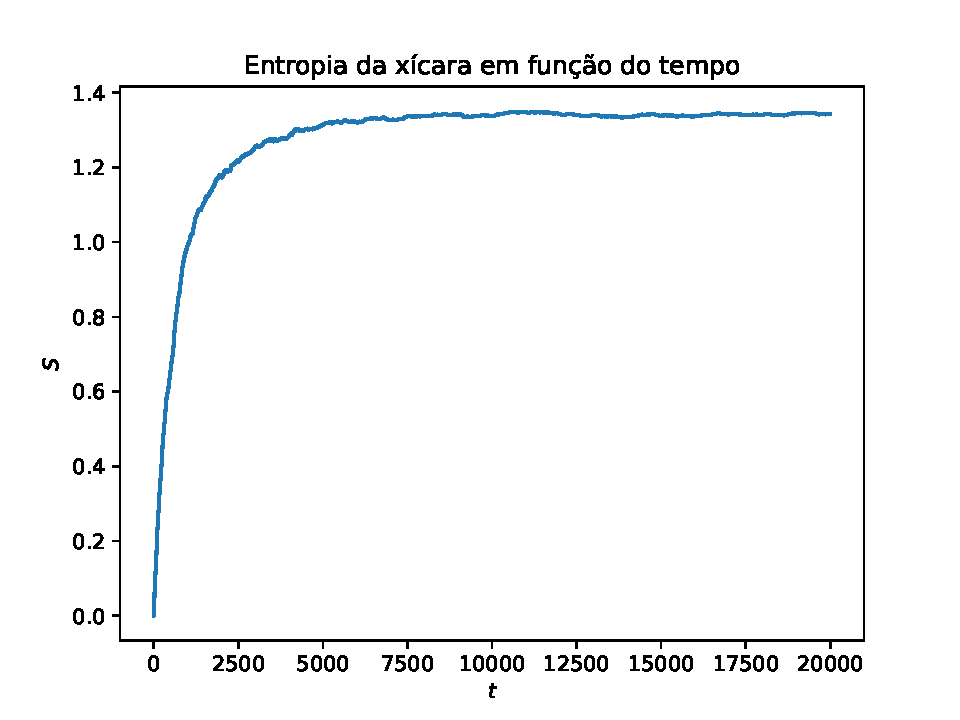
\includegraphics[width=0.4\textwidth]{fig_3b.pdf}
\caption{À esquerda, posições das partículas de creme no café em função do tempo para uma xícara bidimensional \( 11 \times 11 \), com um grid \( 8 \times 8 \), e 1000 partículas. À direita, o gráfico da entropia em função do tempo.}\label{fig3}
\end{figure}

A figura \ref{fig3} apresenta os gráficos que ilustram o café com creme, com a distribuição de partículas para determinados instantes de tempo e com a entropia em função do tempo.
Podemos ver que conforme o sistema entra em equilíbrio termodinâmico, a entropia tende a convergir para um valor aproximadamente igual a \num{1.4}.

\newpage
\section{Exercício 4}

\begin{figure}[ht]
\centering
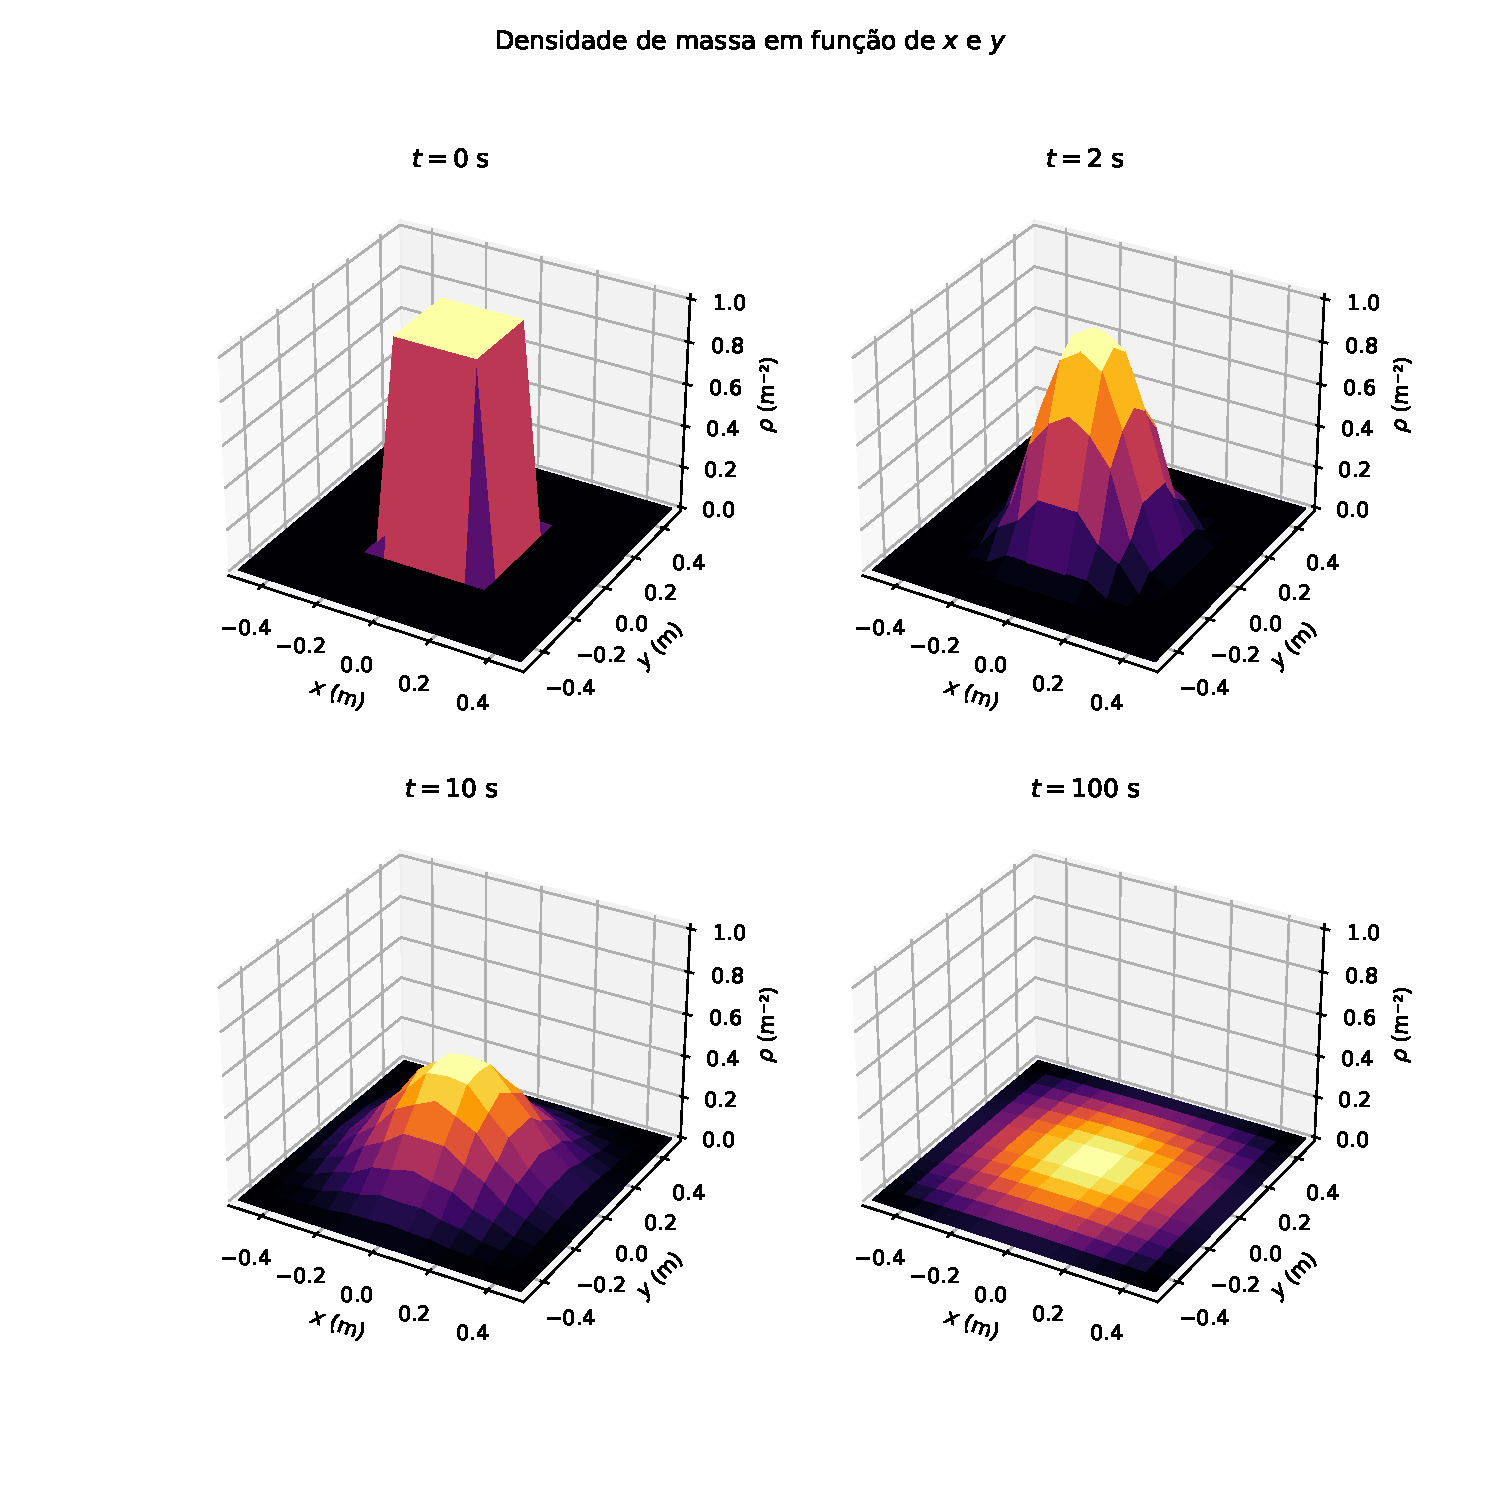
\includegraphics[width=0.45\textwidth]{fig_4a.pdf}
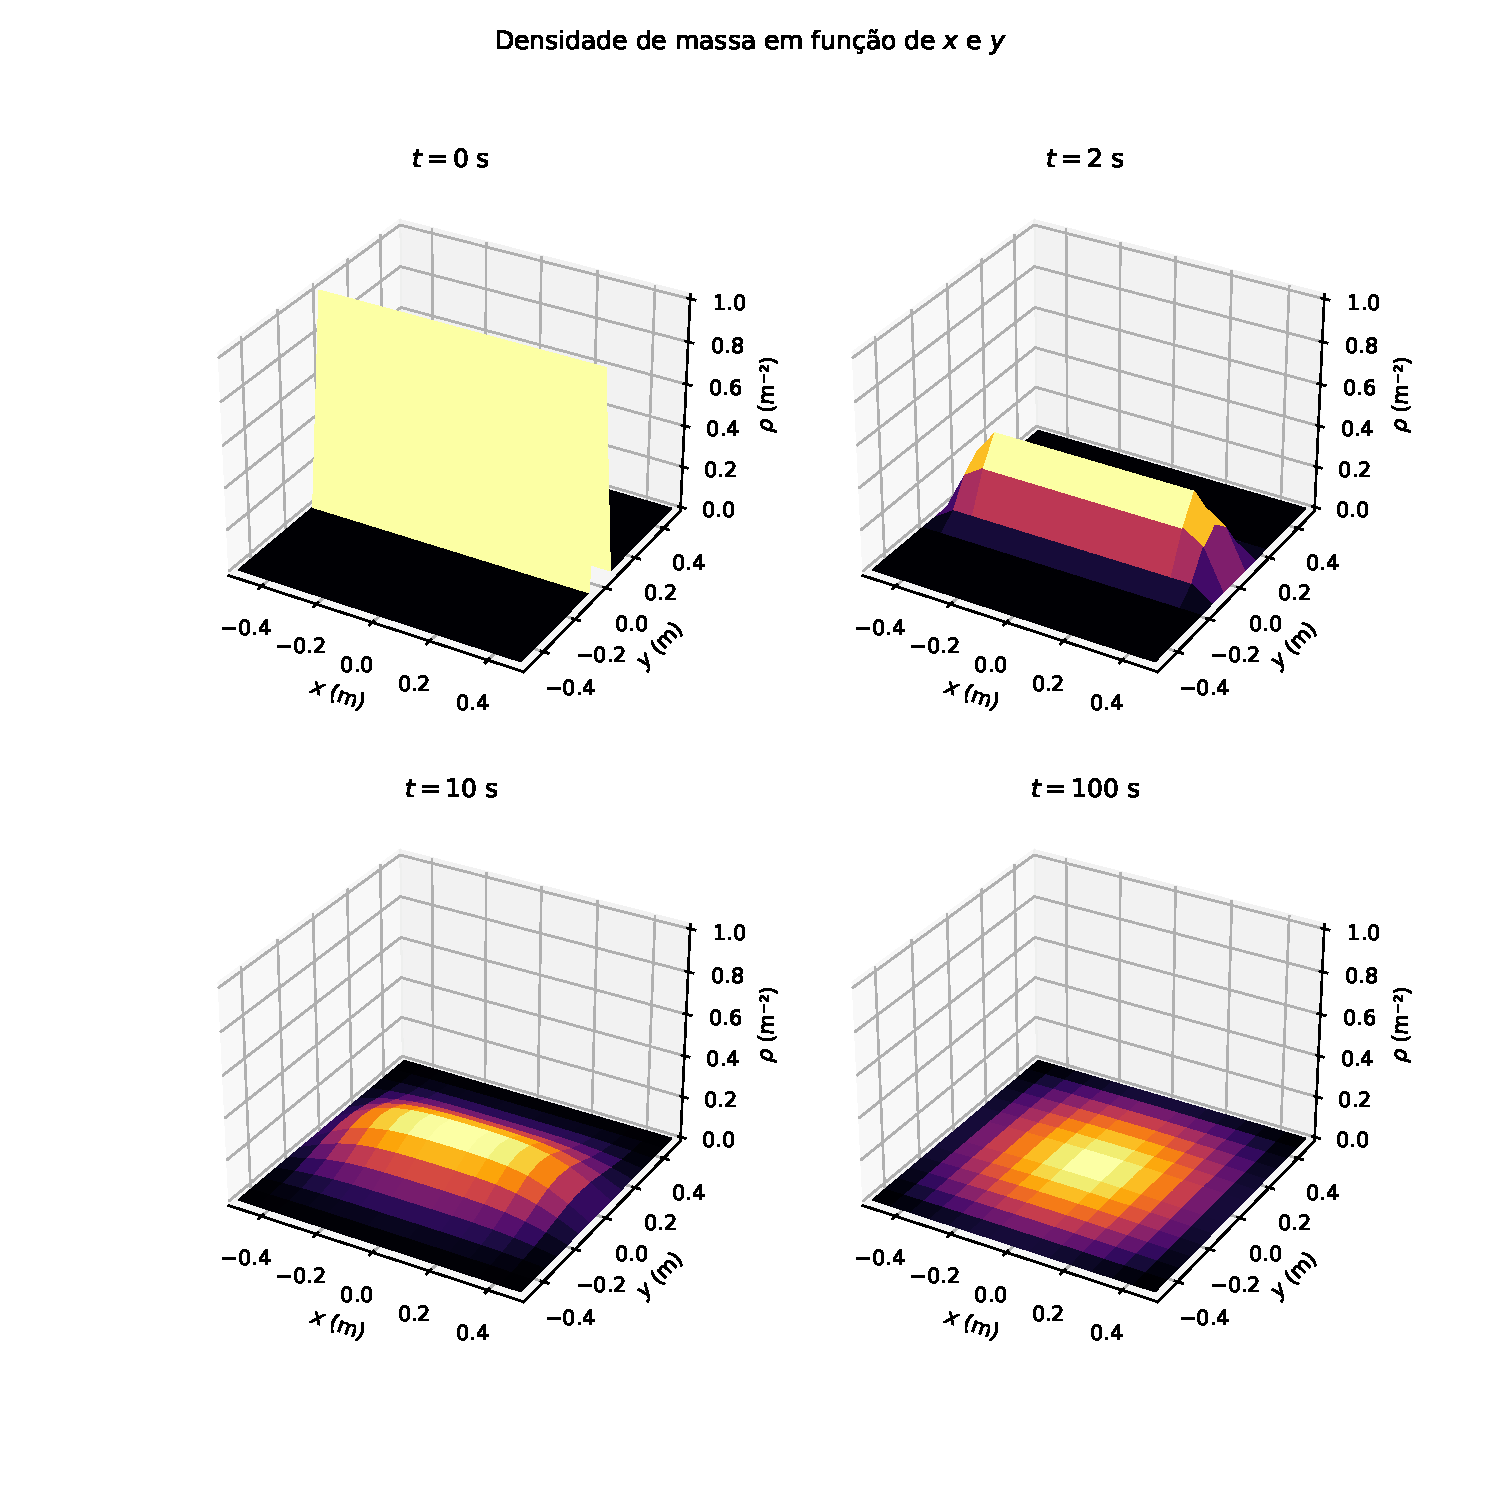
\includegraphics[width=0.45\textwidth]{fig_4b.pdf}
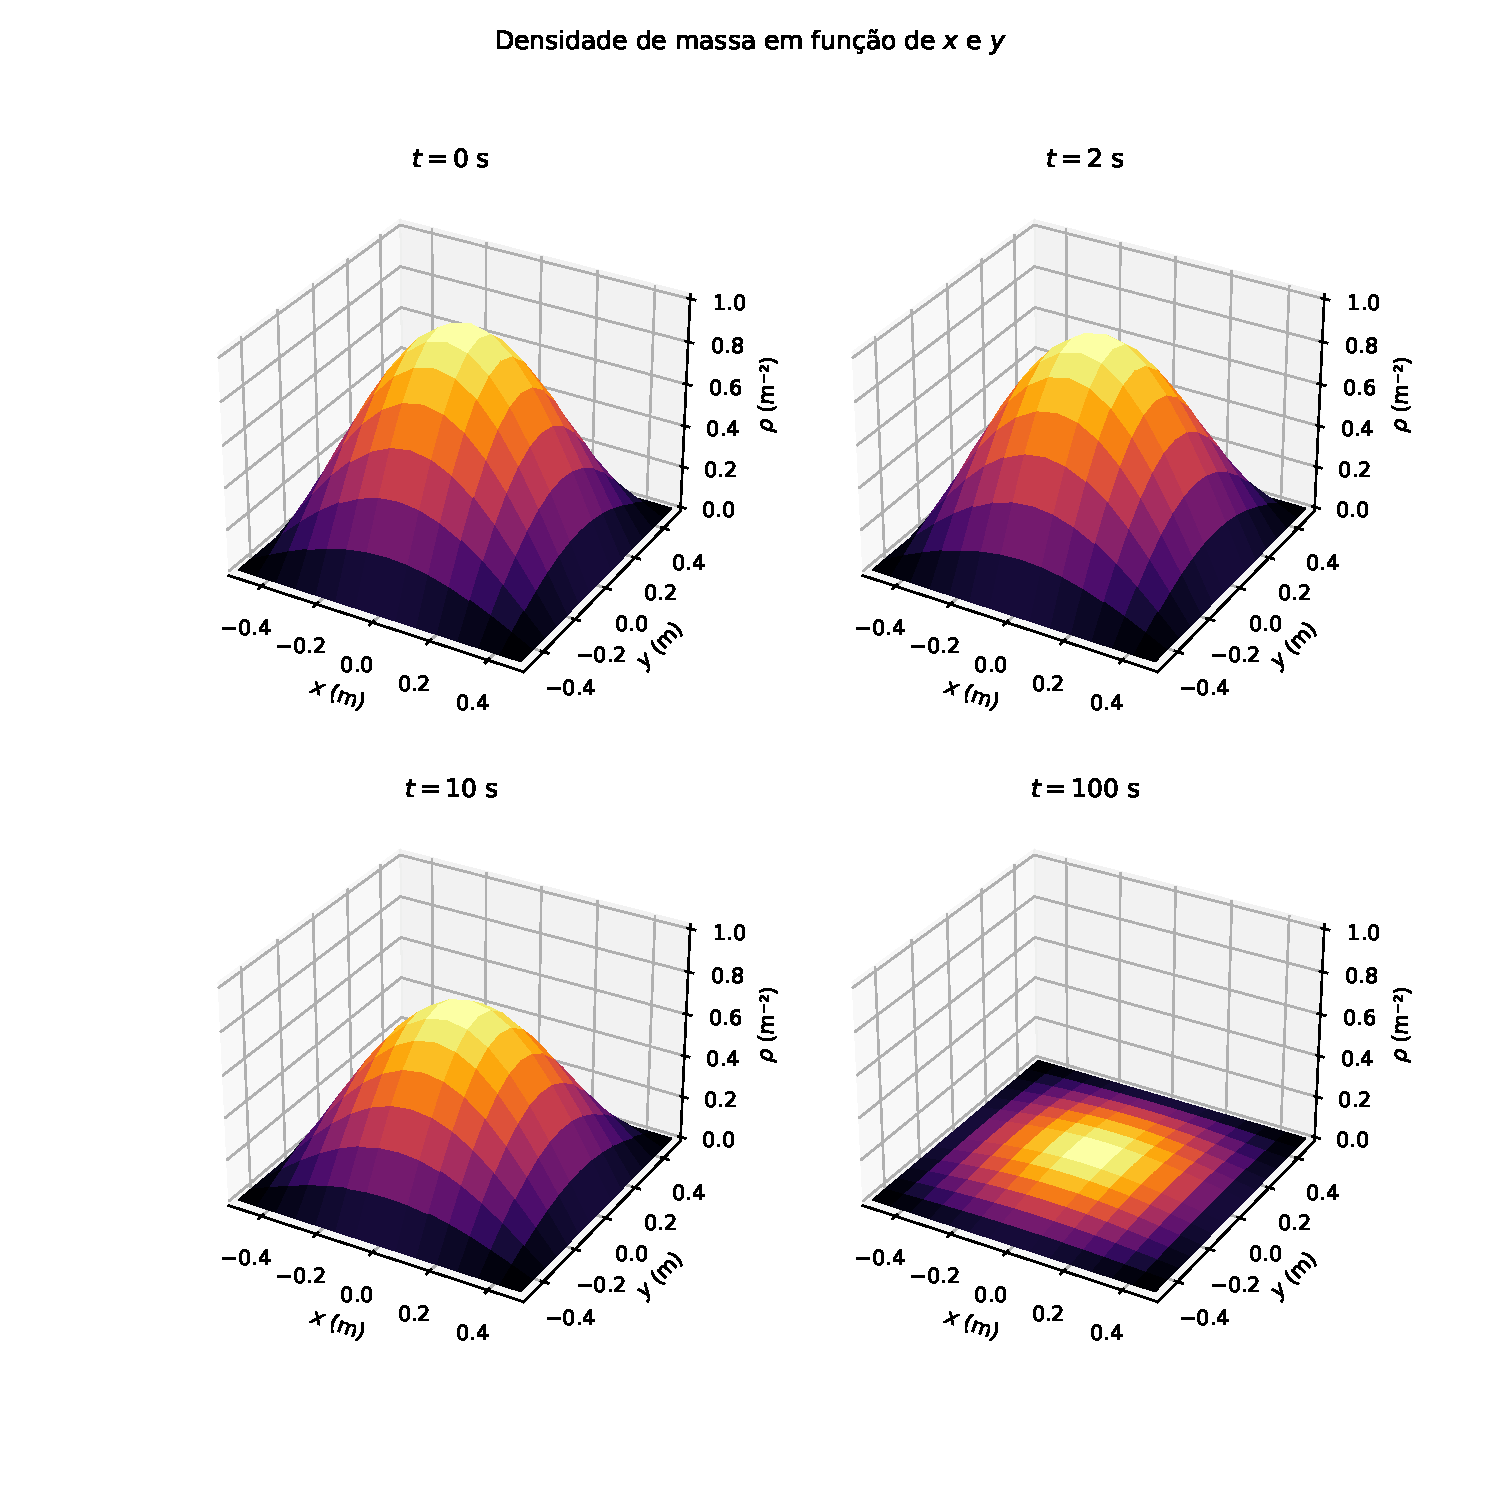
\includegraphics[width=0.45\textwidth]{fig_4c.pdf}
\caption{À esquerda, gráfico da densidade em função do tempo para a distribuição inicial do item a. À direita, gráficos da densidade em função do tempo para a distribuição inicial do item b. Abaixo, gráficos da densidade em função do tempo para a distribuição inicial \( \rho (x, y) = \cos(\pi x) \cos(\pi y) \).}\label{fig4}
\end{figure}

Para todos os itens foi usado um grid 15 por 15, de lados \SI{1}{\meter}.
Para a distribuição do item a, foi escolhido um quadrado de lado \SI{0.3}{\meter}.
Vemos que, para o item a, a distribuição rapidamente se aproxima da função exponencial, como previsto.

\newpage
\section{Exercício 5}

\begin{figure}[ht]
\centering
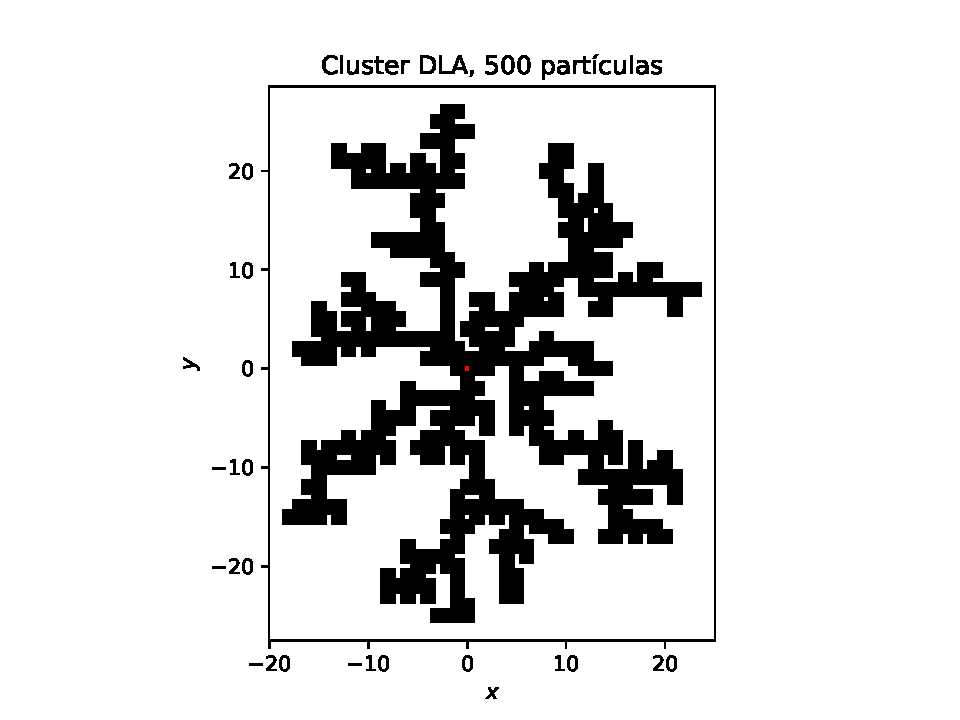
\includegraphics[width=0.4\textwidth]{fig_5a.pdf}
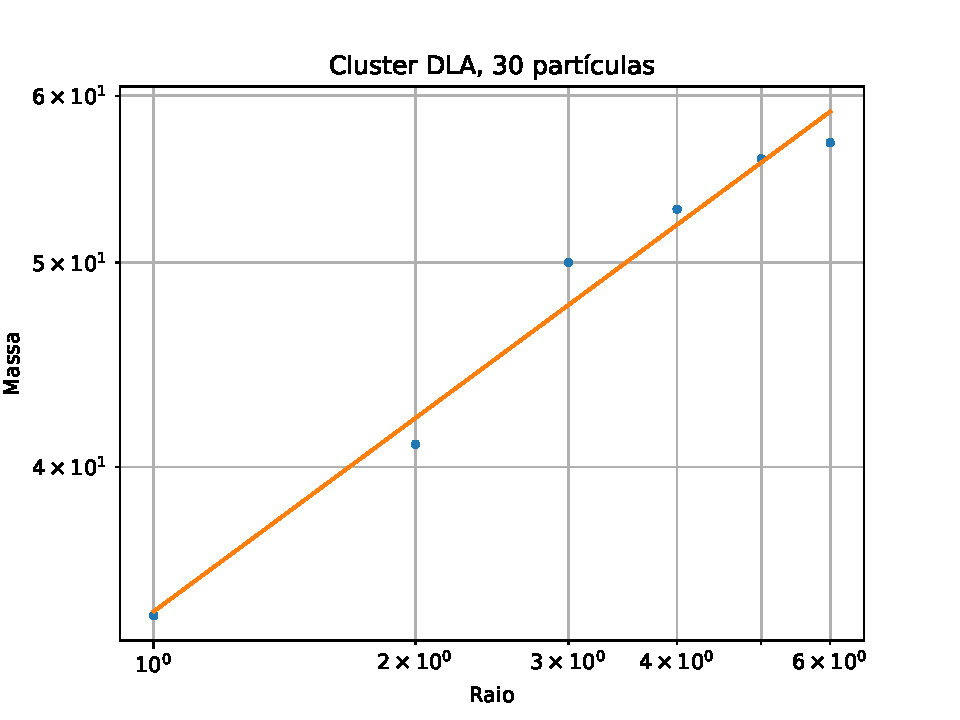
\includegraphics[width=0.4\textwidth]{fig_5b.pdf}
\caption{À esquerda, posições das partículas do agregado DLA. À direita, o gráfico da massa em função do raio, com um ajuste linear para obter a dimensão fractal.}\label{fig5}
\end{figure}

A figura \ref{fig5} apresenta dois gráficos para ilustrar o agregado DLA.
À esquerda, há uma configuração de 500 partículas.
O agregado é gerado da seguinte maneira: uma partícula semente é colocada na origem (em vermelho), e uma posição aleatória num raio de cerca de 5 unidades de distância é escolhida.
A partir dessa posição é iniciado um passeio aleatório bidimensional até que a partícula encontre a vizinhança da semente e grude, ou até que ultrapasse um raio de \( \num{1.5} \times 5 \) unidades de distância, quando o passeio aleatório atual é descartado e um novo é iniciado.
Quando a primeira partícula se grudar, as posições aleatórias a serem sorteadas estarão num raio de 5 vezes o raio máximo do agregado no momento.
Novamente o processo de passeio aleatório é iniciado sob as mesmas regras.
Esse procedimento é repetido até que o agregado tenha o número requerido de partículas.

Ao calcular a massa em função do raio do agregado, podemos obter sua dimensão fractal pelo ajuste linear do gráfico em escala log-log.
Obtive uma dimensão fractal de \num{1.60}, valor próximo ao de \num{1.65}, valor de referência do livro-texto.

\end{document}
